%% Creator: Inkscape inkscape 0.48.0, www.inkscape.org
%% PDF/EPS/PS + LaTeX output extension by Johan Engelen, 2010
%% Accompanies image file 'picSET1+SET2.ps' (pdf, eps, ps)
%%
%% To include the image in your LaTeX document, write
%%   \input{<filename>.pdf_tex}
%%  instead of
%%   \includegraphics{<filename>.pdf}
%% To scale the image, write
%%   \def\svgwidth{<desired width>}
%%   \input{<filename>.pdf_tex}
%%  instead of
%%   \includegraphics[width=<desired width>]{<filename>.pdf}
%%
%% Images with a different path to the parent latex file can
%% be accessed with the `import' package (which may need to be
%% installed) using
%%   \usepackage{import}
%% in the preamble, and then including the image with
%%   \import{<path to file>}{<filename>.pdf_tex}
%% Alternatively, one can specify
%%   \graphicspath{{<path to file>/}}
%% 
%% For more information, please see info/svg-inkscape on CTAN:
%%   http://tug.ctan.org/tex-archive/info/svg-inkscape

\begingroup
  \makeatletter
  \providecommand\color[2][]{%
    \errmessage{(Inkscape) Color is used for the text in Inkscape, but the package 'color.sty' is not loaded}
    \renewcommand\color[2][]{}%
  }
  \providecommand\transparent[1]{%
    \errmessage{(Inkscape) Transparency is used (non-zero) for the text in Inkscape, but the package 'transparent.sty' is not loaded}
    \renewcommand\transparent[1]{}%
  }
  \providecommand\rotatebox[2]{#2}
  \ifx\svgwidth\undefined
    \setlength{\unitlength}{239.32932129pt}
  \else
    \setlength{\unitlength}{\svgwidth}
  \fi
  \global\let\svgwidth\undefined
  \makeatother
  \begin{picture}(1,0.74115818)%
    \put(0,0){\includegraphics[width=\unitlength]{pics/picSET1+SET2.ps}}%
    \put(0.5,0.00484753){\color[rgb]{0,0,0}\makebox(0,0)[lb]{\smash{$r$\,(см)}}}%
    \put(0.012,0.32){\color[rgb]{0,0,0}\rotatebox{90}{\makebox(0,0)[lb]{\smash{$\Delta{}B$\,(мГс)}}}}%
    \put(0.1,0.072){\color[rgb]{0,0,0}\makebox(0,0)[lb]{\smash{$-10$}}}%
    \put(0.31,0.072){\color[rgb]{0,0,0}\makebox(0,0)[lb]{\smash{$-5$}}}%
    \put(0.55310265,0.072){\color[rgb]{0,0,0}\makebox(0,0)[lb]{\smash{$0$}}}%
    \put(0.76080374,0.072){\color[rgb]{0,0,0}\makebox(0,0)[lb]{\smash{$5$}}}%
    \put(0.95563612,0.072){\color[rgb]{0,0,0}\makebox(0,0)[lb]{\smash{$10$}}}%
    \put(0.76916573,0.4592303){\color[rgb]{0,0,0}\makebox(0,0)[lb]{\smash{$(1)$}}}%
    \put(0.79006591,0.56704001){\color[rgb]{0,0,0}\makebox(0,0)[lb]{\smash{$(2)$}}}%
    \put(0.03,0.12174423){\color[rgb]{0,0,0}\makebox(0,0)[lb]{\smash{$-10$}}}%
    \put(0.054,0.2067024){\color[rgb]{0,0,0}\makebox(0,0)[lb]{\smash{$-8$}}}%
    \put(0.054,0.29131385){\color[rgb]{0,0,0}\makebox(0,0)[lb]{\smash{$-6$}}}%
    \put(0.054,0.37590734){\color[rgb]{0,0,0}\makebox(0,0)[lb]{\smash{$-4$}}}%
    \put(0.054,0.46027641){\color[rgb]{0,0,0}\makebox(0,0)[lb]{\smash{$-2$}}}%
    \put(0.094,0.54514819){\color[rgb]{0,0,0}\makebox(0,0)[lb]{\smash{$0$}}}%
    \put(0.094,0.62949931){\color[rgb]{0,0,0}\makebox(0,0)[lb]{\smash{$2$}}}%
    \put(0.094,0.71435313){\color[rgb]{0,0,0}\makebox(0,0)[lb]{\smash{$4$}}}%
  \end{picture}%
\endgroup
